\documentclass[a4paper,12pt]{report} 

\usepackage[italian]{babel} 
\usepackage[utf8]{inputenc} 
\usepackage{graphicx} 
\usepackage{hyperref} 
\usepackage{booktabs} 
\usepackage[backend=biber,style=numeric]{biblatex} 
\usepackage{xcolor} 
\usepackage{geometry} 
\usepackage{titlesec} % Added for section title formatting
\usepackage{url} % Added for better URL formatting

\setcounter{secnumdepth}{1}

% Set page margins
\geometry{
  a4paper,
  total={170mm,257mm},
  left=20mm,
  top=20mm,
}

% Customize section title formatting (adjust as needed)
\titleformat{\section}
  {\Large\bfseries}
  {}
  {0em}
  {}

\begin{document}

% Title and header information (centered and formatted)
\begin{center}
\Large \textbf{Relazione} 

\bigskip

\large Università degli Studi di Milano \\
Corso di Editoria Digitale \\
Anno Accademico 2023-2024 \\
Simone Miglio 978605

\bigskip
\end{center}

\section*{Paris 2024: The Paralympic Games Explained} 

\href{https://github.com/IlDivinatore01/Editoria_Digitale}{Link alla repository del progetto} % Replace with your actual repository URL

\section{Introduzione}

Questo progetto nasce dalla volontà di fornire un'introduzione completa e accessibile ai Giochi Paralimpici di Parigi 2024. L'obiettivo è offrire una panoramica chiara delle diverse discipline sportive, degli atleti straordinari, e dell'impatto culturale e sociale di questo evento globale.

Il progetto mira a raccogliere e integrare informazioni da diverse fonti, inclusi documenti ufficiali, interviste con atleti e allenatori, e risorse online, per creare un'unica risorsa informativa e coinvolgente.

Il formato principale scelto per il prodotto finale è il PDF, per garantire una facile consultazione su dispositivi mobili e e-reader. Il sorgente è stato scritto in LaTeX, sfruttando la sua capacità di gestire testo, immagini e formattazione complessa.  Il tool lualatex è stato utilizzato per convertire il codice sorgente LaTeX in formato EPUB, garantendo un'esperienza di lettura ottimale su diverse piattaforme.

\section{Obiettivi}

L'obiettivo principale di questo PDF è fornire a un pubblico ampio una comprensione approfondita dei Giochi Paralimpici di Parigi 2024. 

I destinatari sono appassionati di sport, studenti, ricercatori, e chiunque sia interessato a conoscere meglio questo evento sportivo unico e il suo impatto sulla società.

Questo ebook si propone di:

\begin{itemize}
    \item Presentare le diverse discipline sportive paralimpiche, spiegandone le regole, le classificazioni e le attrezzature adattate.
    \item Mettere in luce le storie e i successi degli atleti paralimpici, evidenziando la loro determinazione, resilienza e abilità sportive.
    \item Esplorare l'impatto culturale e sociale dei Giochi Paralimpici, promuovendo l'inclusione, l'accessibilità e la parità di opportunità per le persone con disabilità.
    \item Offrire una risorsa completa e accessibile per chiunque desideri approfondire la propria conoscenza dei Giochi Paralimpici di Parigi 2024.
\end{itemize}

\section{Processo di produzione}

\subsection{Studio e analisi del tema}

Il progetto è nato dall'interesse per i Giochi Paralimpici di Parigi 2024 e dalla volontà di creare una risorsa informativa completa ed accessibile su questo evento sportivo. L'obiettivo era quello di andare oltre la semplice cronaca sportiva, esplorando la storia, i valori, le discipline, gli atleti e l'impatto sociale dei Giochi Paralimpici.

La ricerca ha coinvolto la consultazione di diverse fonti, tra cui il sito ufficiale dei Giochi Paralimpici, articoli giornalistici, interviste con atleti e allenatori, e risorse multimediali. L'analisi di questi materiali ha permesso di identificare i temi chiave da trattare e di organizzare i contenuti in modo coerente e strutturato.

\subsection{Definizione del target}

Il target di riferimento per questo ebook è ampio e diversificato. Include appassionati di sport, studenti, ricercatori, e chiunque sia interessato a conoscere meglio i Giochi Paralimpici e il loro significato.

L'ebook si rivolge sia a coloro che hanno già una conoscenza di base dei Giochi Paralimpici, sia a chi si avvicina a questo mondo per la prima volta. L'obiettivo è fornire informazioni chiare e accessibili, stimolando la curiosità e l'interesse verso lo sport paralimpico.

\subsection{Studio competitor}

In questa fase, ho esaminato altre risorse informative sui Giochi Paralimpici, come siti web, articoli e pubblicazioni. Ho notato che molte di queste risorse si concentravano principalmente sulla cronaca sportiva o sugli aspetti organizzativi dell'evento. 

Questo ebook si distingue per la sua volontà di andare oltre, esplorando la storia, i valori, le storie degli atleti e l'impatto sociale dei Giochi, offrendo una prospettiva più completa e coinvolgente.

\subsection{Definizione dei canali e licenze di distribuzione}

L'ebook è stato pubblicato su GitHub sotto licenza Creative Commons Attribution 4.0 International. Questa licenza permette a chiunque di condividere e adattare il materiale, anche per scopi commerciali, purché venga attribuito il merito all'autore originale.

La scelta di questa licenza riflette la volontà di rendere l'ebook il più accessibile possibile, incoraggiando la sua diffusione e il suo utilizzo per scopi educativi e informativi.

\subsection{Identificazione delle fonti}

Le informazioni e i contenuti presenti nell'ebook sono stati raccolti da diverse fonti, tra cui:

\begin{itemize}
\item Il sito ufficiale dei Giochi Paralimpici di Parigi 2024
\item Articoli giornalistici e pubblicazioni specializzate
\item Interviste con atleti, allenatori e organizzatori dei Giochi
\item Risorse multimediali come video e documentari
\item Libri e pubblicazioni accademiche sullo sport paralimpico
\end{itemize}

Tutte le fonti utilizzate sono state citate e referenziate in modo appropriato all'interno del testo e nella bibliografia finale.

\subsection{Definizione dei formati}

La scelta dei formati per la distribuzione dell'ebook è ricaduta sul PDF: è un formato utile per la stampa e la condivisione di documenti, che mantiene la formattazione originale.

Il codice sorgente del PDF è stato scritto in LaTeX, un linguaggio di markup potente e flessibile che permette di gestire testo, immagini, formule matematiche e altri elementi complessi con precisione. 

\subsection{Stesura bozza e revisione dei contenuti}

\subsubsection{Punti da trattare}

La stesura del PDF è iniziata con l'identificazione dei temi chiave da trattare e la loro organizzazione in capitoli e sezioni. 

I contenuti sono stati sviluppati attraverso una ricerca approfondita e l'analisi di diverse fonti, garantendo l'accuratezza e la completezza delle informazioni presentate.

\subsubsection{Sviluppo dei contenuti}

Ogni capitolo è stato redatto con un linguaggio chiaro e accessibile, cercando di bilanciare informazioni dettagliate con una narrazione coinvolgente. 

Sono state inserite immagini, tabelle e altri elementi multimediali per arricchire l'esperienza di lettura e rendere i contenuti più comprensibili.

\subsubsection{Identificazione degli elementi multimediali}

La scelta delle immagini e degli altri elementi multimediali è stata guidata dalla volontà di illustrare i concetti chiave, mostrare l'azione sportiva e raccontare le storie degli atleti paralimpici. 

Tutte le risorse multimediali sono state selezionate e utilizzate nel rispetto del copyright e delle normative vigenti.

\subsubsection{Revisione}

Il documento è stato sottoposto a un'attenta revisione per garantire la correttezza grammaticale, la chiarezza espositiva e la coerenza stilistica. 

È stata inoltre verificata l'accuratezza delle informazioni e delle fonti citate.

\section{Definizione dello stile grafico}

La formattazione del testo, l'impaginazione e l'aspetto grafico del PDF sono stati curati con attenzione per garantire una lettura piacevole e coinvolgente. LaTeX, il linguaggio di markup utilizzato per la creazione del sorgente, ha offerto un controllo preciso sulla presentazione dei contenuti, assicurando un risultato professionale e coerente.

Sono stati scelti font chiari e leggibili, con dimensioni adeguate per favorire la lettura su diversi dispositivi. L'impaginazione è stata studiata per creare un equilibrio visivo tra testo, immagini e altri elementi grafici, evitando affollamenti e facilitando la navigazione all'interno dell'ebook. 

I colori principali dei Giochi Paralimpici (rosso, blu e verde) sono stati utilizzati per evidenziare il titolo, creando un legame visivo con il tema dell'ebook.

\section{Gestione Documentale}

La gestione documentale in questo progetto ha coinvolto l'organizzazione e il controllo dei vari file e risorse utilizzati per la creazione dell'ebook. È stata adottata una struttura di cartelle chiara e intuitiva per facilitare la navigazione e l'individuazione dei diversi elementi del progetto.

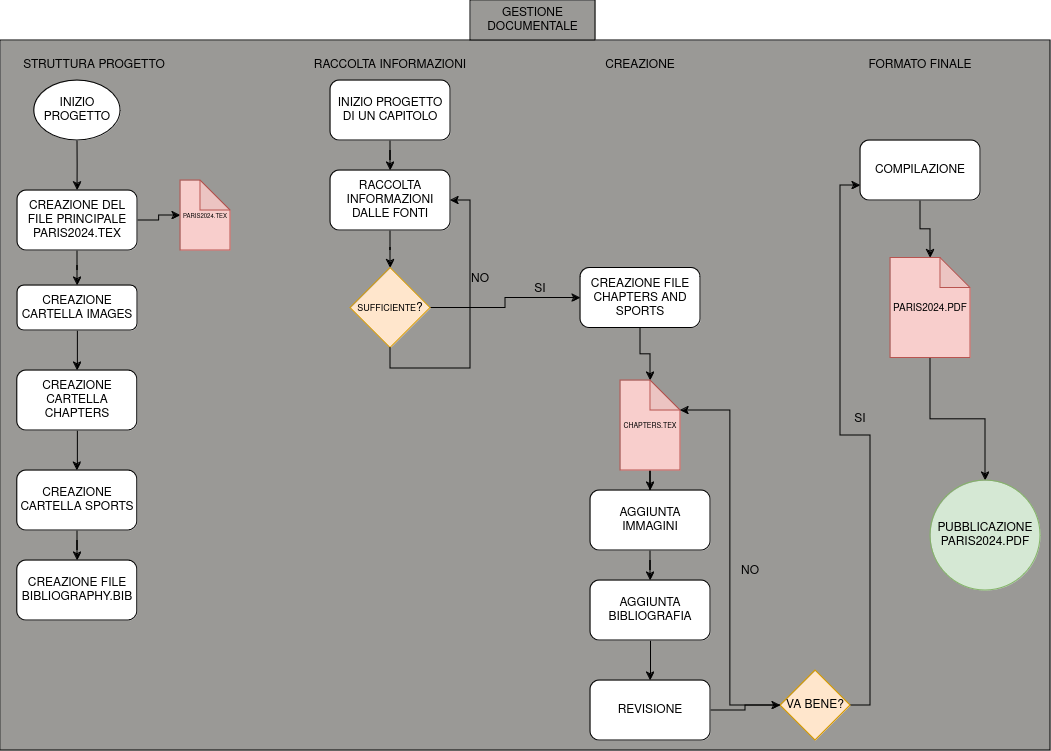
\includegraphics[width=1\textwidth]{GestioneDocumentale.png}

\subsection{Struttura delle cartelle}

Il progetto è stato organizzato in diverse cartelle per mantenere i file ben strutturati e separati in base alla loro funzione:

\begin{itemize}
\item `chapters/`: Contiene i file `.tex` dei singoli capitoli dell'ebook.
\item `images/`: Contiene tutte le immagini utilizzate nell'ebook.
\item `sports/`: Contiene i file `.tex` delle sottosezioni relative alle singole discipline sportive, inclusi nel capitolo "Sport e Categorie".
\end{itemize}

\subsection{Gestione delle immagini}

Le immagini sono state inserite nel documento LaTeX utilizzando il pacchetto `graphicx` e il comando `\ includegraphics`. 

Per garantire la corretta visualizzazione delle immagini sia nel PDF che nell'EPUB, sono state seguite queste linee guida:

\begin{itemize}
\item Formati supportati: Le immagini sono state salvate in formati compatibili con entrambi i formati di output, come JPEG o PNG.
\item Percorsi relativi: I percorsi delle immagini sono stati specificati in modo relativo alla posizione del file `Main.tex` per evitare problemi durante la compilazione e la conversione.
\item Dimensioni e posizionamento: Le dimensioni e il posizionamento delle immagini sono stati controllati utilizzando le opzioni del comando `\ includegraphics` per garantire una visualizzazione ottimale.
\end{itemize}

\subsection{Bibliografia}

La bibliografia è stata gestita utilizzando il pacchetto `biblatex` con il backend Biber. Le informazioni bibliografiche sono state raccolte in un file `references.bib` in formato BibTeX.

Le citazioni all'interno del testo sono state inserite utilizzando il comando `\ cite`, e la bibliografia finale è stata generata automaticamente alla fine dell'ebook grazie al comando `\ printbibliography`.

\subsection{Controllo di versione con Git e GitHub}

Il sistema di controllo di versione Git, integrato con la piattaforma GitHub, è stato utilizzato per tenere traccia delle modifiche apportate al codice sorgente LaTeX, alle immagini e ad altri file. 
Grazie a Git, è stato possibile:

\begin{itemize}
\item Versionare il progetto: Mantenere una cronologia completa delle modifiche, consentendo di tornare a versioni precedenti in caso di necessità.
\item Collaborare in modo efficiente: Facilitare la collaborazione tra più persone sul progetto, gestendo le modifiche apportate da ciascun membro del team.
\item Condividere il progetto: Rendere il codice sorgente e le risorse accessibili pubblicamente su GitHub, favorendo la trasparenza e la possibilità di contributi esterni.
\end{itemize}

L'utilizzo di Git e GitHub ha permesso di gestire il progetto in modo organizzato e controllato, garantendo la tracciabilità delle modifiche e facilitando la collaborazione e la condivisione del lavoro.

\section{Creazione del formato di distribuzione}

Una volta completata la stesura e la revisione dei contenuti, il codice sorgente LaTeX è stato compilato utilizzando LuaLaTeX per generare un file PDF. LuaLaTeX è stato scelto per la sua capacità di gestire l'incorporazione di elementi multimediali, come le immagini, all'interno del PDF.

Il risultato finale è un ebook in formato PDF, completo di immagini, formattazione accurata e collegamenti ipertestuali, che offre un'esperienza di lettura coinvolgente e accessibile su diverse piattaforme.

\section{Tecnologie Adottate}

Di seguito sono elencate le tecnologie utilizzate per la realizzazione di questo ebook, insieme a una breve descrizione del loro ruolo nel processo di sviluppo.

\begin{itemize}
	\item LaTeX
	\item make
	\item GitHub
\end{itemize}

\subsection{LaTeX}

LaTeX è stato scelto come linguaggio di markup principale per la creazione del contenuto dell'ebook. I motivi principali di questa scelta includono:

\begin{itemize}
	\item \textbf{Qualità tipografica:}** LaTeX offre un'eccellente gestione della tipografia, garantendo un risultato professionale e di alta qualità per l'ebook.
	\item \textbf{Strutturazione dei contenuti:}** LaTeX facilita l'organizzazione dei contenuti in capitoli, sezioni e sottosezioni, consentendo una chiara strutturazione dell'ebook.
	\item \textbf{Gestione di elementi complessi:}** LaTeX gestisce in modo efficiente tabelle, figure, formule matematiche e altri elementi complessi, essenziali per presentare informazioni in modo chiaro e organizzato.
	\item \textbf{Automazione:}** LaTeX automatizza molti aspetti della formattazione, come la generazione dell'indice dei contenuti, la numerazione delle pagine e la gestione dei riferimenti incrociati, semplificando il processo di creazione dell'ebook.
	\item \textbf{Flessibilità e personalizzazione:}** LaTeX offre un'ampia gamma di pacchetti e opzioni per personalizzare l'aspetto dell'ebook, consentendo di adattare lo stile grafico alle esigenze specifiche del progetto.
\end{itemize}
					
Per lo sviluppo di questo progetto è stato utilizzato l'editor TeXstudio su sistema operativo Windows. 
					
La struttura del codice LaTeX è organizzata in un file principale (`Main.tex`) che include i singoli capitoli tramite il comando `\ include`. Il file principale contiene anche le impostazioni generali del documento, come il titolo, l'autore, la data e le informazioni sul copyright.
					
Alcuni dei pacchetti LaTeX utilizzati in questo progetto includono:
					
\begin{itemize}
	\item \textbf{graphicx:} Per la gestione dell'inclusione e del posizionamento delle immagini.
	\item \textbf{hyperref:} Per la creazione di collegamenti ipertestuali e la gestione dei segnalibri all'interno dell'ebook.
	\item \textbf{booktabs:} Per la creazione di tabelle di alta qualità con una formattazione professionale.
	\item \textbf{biblatex:} Per la gestione della bibliografia e delle citazioni all'interno del testo.
	\item \textbf{xcolor:} Per la gestione dei colori, in particolare per l'utilizzo dei colori ufficiali dei Giochi Paralimpici nella copertina.
	\item \textbf{geometry:} Per la personalizzazione dei margini e delle dimensioni della pagina.
	\item \textbf{titlesec:} Per la formattazione dei titoli di sezione e sottosezione.
\end{itemize}
					
Per la compilazione del codice sorgente LaTeX e la generazione del file PDF è stato utilizzato il motore LuaLaTeX. Questo motore è stato scelto per la sua capacità di gestire l'incorporazione di elementi multimediali, come video e audio, all'interno del PDF, e per la sua compatibilità con i font OpenType.
					
Il comando utilizzato per la compilazione è il seguente:
					
```bash
lualatex -interaction=nonstopmode -output-directory=build -jobname=Paris2024 Main.tex
					
\subsection{make}
					
Make è un'utility che automatizza il processo di compilazione e conversione del documento. Grazie a un file Makefile, è possibile definire le dipendenze tra i vari file del progetto e i comandi necessari per generare i diversi formati di output.
					
Nel contesto di questo progetto, il Makefile permette di ompilare il codice sorgente LaTeX in PDF utilizzando LuaLaTeX.
					
L'utilizzo di make semplifica e velocizza il processo di creazione dell'ebook, soprattutto quando si apportano modifiche al codice sorgente o si aggiungono nuovi contenuti.
					
\subsection{GitHub}
					
GitHub è una piattaforma di sviluppo software basata sul sistema di controllo di versione Git. In questo progetto, GitHub è stato utilizzato per:
					
\begin{itemize}
	\item \textbf{Archiviazione e versionamento del codice:}** Il codice sorgente LaTeX, le immagini, i file audio e il Makefile sono stati archiviati nel repository GitHub, consentendo di tenere traccia delle modifiche e delle diverse versioni del progetto.
	\item \textbf{Collaborazione:}** GitHub offre strumenti per la collaborazione tra più persone sullo stesso progetto, facilitando la condivisione del codice e la gestione delle modifiche.
	\item \textbf{Distribuzione:}** Il repository GitHub funge da punto di accesso pubblico all'ebook, consentendo a chiunque di scaricare il codice sorgente o il file PDF finale.
\end{itemize}
						
L'utilizzo di GitHub ha reso il progetto più trasparente, accessibile e collaborativo, favorendo la diffusione dell'ebook e la possibilità di migliorarlo ulteriormente grazie al contributo di altri utenti.
								
\section{Conclusioni}

L'ebook realizzato, "Paris 2024: The Paralympic Games Explained", ha raggiunto gli obiettivi prefissati, offrendo una panoramica completa e coinvolgente dei Giochi Paralimpici di Parigi 2024.

Il prodotto finale si presenta come una risorsa informativa preziosa per chiunque desideri approfondire la propria conoscenza di questo evento sportivo. L'ebook esplora la storia, i valori, le discipline, gli atleti e l'impatto sociale dei Giochi, fornendo un quadro completo e stimolante.

La struttura chiara e organizzata, l'uso di immagini e altri elementi multimediali, e la formattazione curata contribuiscono a rendere l'ebook piacevole da leggere e di facile consultazione. La presenza di un indice dei contenuti interattivo facilita la navigazione e la ricerca di informazioni specifiche.

Tuttavia, sono consapevole che ci sono margini di miglioramento. Ad esempio, l'integrazione di video e altri contenuti multimediali interattivi potrebbe arricchire ulteriormente l'esperienza di lettura e rendere il PDF ancora più coinvolgente.

In futuro, sarebbe interessante tramite il comando pandoc creare un file .epub, utile per i dispositivi come Kindle e Kobo.

Nonostante questi possibili miglioramenti, ritengo che l'ebook "Paris 2024: The Paralympic Games Explained" rappresenti un contributo significativo alla diffusione della conoscenza e della consapevolezza sui Giochi Paralimpici. Spero che questo progetto possa ispirare e informare un vasto pubblico, promuovendo l'inclusione e la valorizzazione delle abilità di tutti gli atleti.
								
\end{document}
